\hypertarget{group___bilinear_interpolate}{}\section{Bilinear Interpolation}
\label{group___bilinear_interpolate}\index{Bilinear Interpolation@{Bilinear Interpolation}}
Collaboration diagram for Bilinear Interpolation\+:
\nopagebreak
\begin{figure}[H]
\begin{center}
\leavevmode
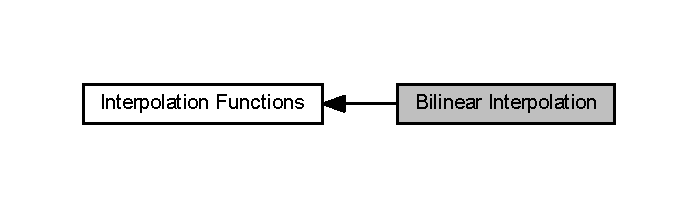
\includegraphics[width=335pt]{group___bilinear_interpolate}
\end{center}
\end{figure}


\subsection{Detailed Description}
Bilinear interpolation is an extension of linear interpolation applied to a two dimensional grid. The underlying function {\ttfamily f(x, y)} is sampled on a regular grid and the interpolation process determines values between the grid points. Bilinear interpolation is equivalent to two step linear interpolation, first in the x-\/dimension and then in the y-\/dimension. Bilinear interpolation is often used in image processing to rescale images. The C\+M\+S\+IS D\+SP library provides bilinear interpolation functions for Q7, Q15, Q31, and floating-\/point data types.

{\bfseries Algorithm} \begin{DoxyParagraph}{}
The instance structure used by the bilinear interpolation functions describes a two dimensional data table. For floating-\/point, the instance structure is defined as\+: 
\begin{DoxyPre}
  typedef struct
  \{
    uint16\_t numRows;
    uint16\_t numCols;
    float32\_t *pData;
\} \hyperlink{structarm__bilinear__interp__instance__f32}{arm\_bilinear\_interp\_instance\_f32};
\end{DoxyPre}

\end{DoxyParagraph}
\begin{DoxyParagraph}{}
where {\ttfamily num\+Rows} specifies the number of rows in the table; {\ttfamily num\+Cols} specifies the number of columns in the table; and {\ttfamily p\+Data} points to an array of size {\ttfamily num\+Rows$\ast$num\+Cols} values. The data table {\ttfamily p\+Table} is organized in row order and the supplied data values fall on integer indexes. That is, table element (x,y) is located at {\ttfamily p\+Table\mbox{[}x + y$\ast$num\+Cols\mbox{]}} where x and y are integers.
\end{DoxyParagraph}
\begin{DoxyParagraph}{}
Let {\ttfamily (x, y)} specify the desired interpolation point. Then define\+: 
\begin{DoxyPre}
    XF = floor(x)
    YF = floor(y)
\end{DoxyPre}
 
\end{DoxyParagraph}
\begin{DoxyParagraph}{}
The interpolated output point is computed as\+: 
\begin{DoxyPre}
 f(x, y) = f(XF, YF) * (1-(x-XF)) * (1-(y-YF))
          + f(XF+1, YF) * (x-XF)*(1-(y-YF))
          + f(XF, YF+1) * (1-(x-XF))*(y-YF)
          + f(XF+1, YF+1) * (x-XF)*(y-YF)
\end{DoxyPre}
 Note that the coordinates (x, y) contain integer and fractional components. The integer components specify which portion of the table to use while the fractional components control the interpolation processor.
\end{DoxyParagraph}
\begin{DoxyParagraph}{}
if (x,y) are outside of the table boundary, Bilinear interpolation returns zero output. 
\end{DoxyParagraph}
